\documentclass[]{article}
\usepackage{multicol}
\usepackage[margin = 1.25in]{geometry}
\usepackage{graphicx}
\usepackage{mathtools}
\usepackage{caption}
\usepackage{lipsum}
\usepackage{algpseudocode}
\usepackage{fancyvrb}
\usepackage{amsfonts}
\usepackage{amsmath}
\usepackage{textcomp}
\newenvironment{Figure}
  {\par\medskip\noindent\minipage{\linewidth}}
  {\endminipage\par\medskip}

\usepackage{setspace}
\linespread{2.0}
\setlength{\parskip}{1em}

\newtheorem{theorem}{Theorem}[section]
\newtheorem{lemma}[theorem]{Lemma}
\newtheorem{proposition}[theorem]{Proposition}
\newtheorem{corollary}[theorem]{Corollary}

\newenvironment{proof}[1][Proof]{\begin{trivlist}
\item[\hskip \labelsep {\bfseries #1}]}{\end{trivlist}}
\newenvironment{definition}[1][Definition]{\begin{trivlist}
\item[\hskip \labelsep {\bfseries #1}]}{\end{trivlist}}
\newenvironment{example}[1][Example]{\begin{trivlist}
\item[\hskip \labelsep {\bfseries #1}]}{\end{trivlist}}
\newenvironment{remark}[1][Remark]{\begin{trivlist}
\item[\hskip \labelsep {\bfseries #1}]}{\end{trivlist}}

\newtheorem{hyp}{Hypothesis}

\makeatletter
\newcounter{subhyp} 
\let\savedc@hyp\c@hyp
\newenvironment{subhyp}
 {%
  \setcounter{subhyp}{0}%
  \stepcounter{hyp}%
  \edef\saved@hyp{\thehyp}% Save the current value of hyp
  \let\c@hyp\c@subhyp     % Now hyp is subhyp
  \renewcommand{\thehyp}{\saved@hyp\alph{hyp}}%
 }
 {}
\newcommand{\normhyp}{%
  \let\c@hyp\savedc@hyp % revert to the old one
  \renewcommand\thehyp{\arabic{hyp}}%
} 
\makeatother


%opening
\title{Modeling Network User Behavior: Probabilistic Programming and Beyond}
\date{May 13, 2016}
\author{Shidan Xu}


\begin{document}
\maketitle

%\begin{abstract}
%
%\end{abstract}



\begin{abstract}

This paper describes a Master of Engineering project at the MIT Advanced Networks Architecture (ANA) group. This project involves learning to predict users' mobility within the network topology. This topological mobility, as opposed to physical mobility, can be substantial as the user switches from LTE to wireless network, while moving minimally physically. Our dataset consists of email IMAP logs as they document associated client IP addresses, as well as the clients' identifiers. Prediction for online mobility is of particular interest to the networks community. If we can predict online mobility with high probability, then new network architecture can be designed to optimize the caching system by minimizing resending packets.  We used various approaches and techniques to model the user's behavior, including probabilistic programming, regression, neural nets, and clustering algorithms. We compare and contrast how different models differ in their prediction accuracy, speed of convergence, and complexity. 

Thesis Supervisor: Dr. Karen Sollins and Dr. Steven Bauer.

\end{abstract}
%This paper describes a thesis project at the MIT Advanced Networks Architecture (ANA) group. This project involves predicting a user's behavior in various networks. In particular, we are interested in how the user is likely to transition between networks. We plan to design various models to predict the user's behavior, and use various evaluation criteria to understand which model most vividly captures the user's behavior. As a learning experience for our team and me, we employ probabilistic programming (PP) techniques. PP is a way of programming that utilizes existing software packages that include encapsulated methods for the inference step of machine learning. By simplifying the implementation, it allows researchers to focus on models. This project has two main objectives. The first is to design several models to capture one or multiple aspects of a typical user, or a group of users' behavior in a network. The second is to evaluate each model to decide which model is more feasible, and which model is applicable under what situations. Together this project aims to give a better understanding of how network user transitions.


\newpage


\section*{Acknowledgement}

I would like to thank Dr. Karen Sollins and Dr. Steven Bauer for giving me an opportunity to work on this MobilityFirst project for my MEng. I loved my time exploring the intricacies in the datasets and I learned so much in the research process.

I would like to thank Dr. Karen Sollins and Dr. Steven Bauer for their continued advice and insight into conceiving this project and thesis.

I would like to thank Dr. Bauer for his technical help and project focus guidance throughout this project. I'd like to thank Dr. Sollins for all of her help with design decisions and project planning. Without their insights, this project would not have been possible. Their help was invaluable.

I would like to thank Tingtao Zhou, Tianfan Xue, and Zhengli Wang for their help with the statistics concepts and machine learning ideas.

Lastly, I would like to thank my family for all of their support, love, and help in life. 

This project was funded in part under NSF Grant 1413973, "NeTS: Large: Collaborative Research: Location-Independent Networks: Evaluation Strategies and Studies".


\newpage
\singlespacing
\tableofcontents
\newpage
\listoffigures
\listoftables

\doublespacing
\linespread{2.0}
\selectfont

\newpage

\section{Introduction}

\subsection{Project Background}

The Internet is approaching a historic inflection point, with mobile platforms and applications replacing the fixed-host/server model that has dominated the Internet since its inception \cite{mobilityfirst}. This gradual shift produces an opportunity to design a new network focused on mobile users. This project relates to the MobilityFirst project in the FIND (Future Internet Design) initiative \cite{find}, which asks the question of what the requirements should be for a global network 15 years from now, and how we can build such a network if we are not constrained by the current Internet. 

\subsection{Current Internet Has Inefficiency}
Developers of the Internet made some design choices with assumptions. One particular assumption is that network mobility is similar to mobility in geography\cite{jacobson}. However, in real world cases, we found that assumption to be increasingly often violated. For example, a phone user could transition from a 4G network to Wi-Fi by walking a few meters in real world, but the IP addresses in network topology are likely to be not adjacent, even entirely different. In extreme cases, the nearest common ancestor of nodes in network topology can be on opposite coasts of the country. Such design is costly for the user to transition between networks. In designing a new network, one of the focal points is to decrease such inconsistency, as packets of information need to be rerouted. The future network needs to address this geologically proximate network change, and maximize the efficiency for such data transfer.

\begin{Figure}
 \centering
 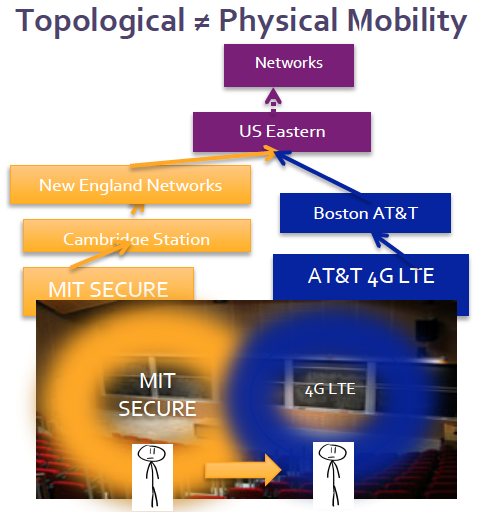
\includegraphics[height = 11cm, width =10cm]{topneqphy.png}
 \captionof{figure}{Topological mobility is not equal to physical mobility. The nearest common ancestor for the 4G LTE network and the MIT network goes all the way up to US Eastern.}
\end{Figure}

Imagine a person traversing through a college campus while checking his email on the phone. As he moves along, his phone's network switches from LTE and his college network alternatively. Every time the user switches network, his phone loses some data and has to send extra requests to recover lost data. The LTE and campus wifi, despite being geologically close by, can be vastly distant in network topology. Hence a request may have to go up multiple layers, before finally reaching a common ancestor. This extra path traversed carries inefficiency in the current network. 

Consider another typical 9-5 office worker. She wakes up at 8, goes to work at 9, comes home at 5. She has dinner at 6 and spends two hours surfing the web at night. Now consider how her daily network usage would look like. She would be on her home network in the morning. She uses a combination of the company and LTE network at work. Sometimes she eats lunch at a coffee shop and uses the network there. She spends some time on her home network at night. Her active network traffic ends at 11, but some passive email checking and other maintenance from her device persist throughout the night. Her daily network usage is very predictable. If researchers can predict her network usage, notifications can be customized to make her life more convenient. 

Multiple questions can be asked in those two scenarios. To what accuracy is human network behavior habitual? To what degree can user network behavior be predicted? How should we evaluate network usage behavior? How often do such costly network transitions happen? How do we measure the cost of one such transition? How much traffic is affected by those costly transitions? How should we design our networks to avoid this costly transition?

\subsection{Understand User Transition Behavior}

This project focuses on understanding the users' transition behavior, as opposed to evaluating network usage. Two main reasons support the decision. 1. Networks are designed to advance knowledge across the spectrum of human endeavors\cite{netsfia}, to facilitate daily life, not vice versa. 2. Studying from the networks perspective increases difficulty in discovering mobility. A network can provide information on who is currently utilizing the network, but does not see the user in a chronological perspective, especially whenever s/he is not on this particular network. 

\subsection{Relations to MobilityFirst}
The MobilityFirst projects presents several major design goals \cite{mobilityfirst}:

\begin{itemize}
\item
Dynamic hosting to provide scalable network mobility.
\item
The robustness of the wireless transfer medium.
\item
Reinforce network security and privacy for both mobile and wired networks.
\item
Provide context-aware mobile services.
\end{itemize}

By investigating the users behavioral trend, this project aims to gain a comprehensive understanding on when the current Internet design would benefit from dynamic hosting.

\subsection{Data Analysis Approaches on Networks Problem}

Additionally, the project stresses to create a procedure for quick turnaround of modeling using approaches such as probabilistic programming and neural nets. These procedures are chosen to quickly expand on the current model. The researcher spent time in evaluating the different approaches and tools for their performance. 

Noam Chomsky believed that the Merge operation is one of the fundamental differences that separate humans apart from other primates \cite{whyonlyus}. That is, humans can take two abstract concepts and combine them to create scenarios that s/he has never physically experienced. A person can imagine a dinosaur ripping apart an opera stage as long as he understands dinosaurs and opera, despite he has never seen such an event in reality. This Merge ability can induce creativity. In the networks community, research on evaluation of network architecture is sometimes qualitative (SOURCE?). Statistical methods and machine learning are trending approaches to extract insight out of the dataset. By applying machine learning strategies to a networks problem, we try to develop new insight that's not traditionally seen.

\newpage

\section{Previous Works on Quantitative Network Measurements}

\subsection{Sookhyun Yang's Three State Markov Model}


We based our work on Yang's Measurement and Modeling of User Transition Among Networks \cite{yang}. 

Yang's paper created a 3-state Markov model that's evaluated by measuring the distribution of cost function of signaling a network attachment / detachment, using Internet Message Access Protocol (IMAP) logs for email access for the population of University of Massachusetts at Amherst residents \cite{yang}. 

\subsubsection{Choosing the Dataset}

A major difficulty in networks mobility research is to select a dataset that captures user transitions. Yang argued for three major criteria for selecting a proper dataset\cite{yang}. 

\begin{itemize}
\item
The application should be frequently used by the user to provide a sufficiently large dataset.
\item
The application can be monitored without introducing extra hurdle.
\item
The application provides trackable user identification.
\end{itemize}

Therefore, Yang's choice on IMAP logs is a good exploration that satisfies those requirements. We also had several options choosing our datasets.

\begin{itemize}
\item
Use the Yang dataset, but with limited columns due to privacy control.
\item
Collect our own email based dataset.
\item
Use mobility datasets from a third party provider such as Sprint.
\end{itemize}

If we pick Yang's dataset, we have a leap ahead into what kind of approaches we can take to understand the dataset. More importantly, we save time in acquiring the dataset ourselves, which in Yang's case took four entire months. The cons include that the user identity is masked due to privacy concerns, and each data entry has limited content. The following is an example of what the Yang dataset looks like. We can also collect our own email-based dataset at MIT. In order to extract more information on the user's age, residence, etc., we need to clear privacy controls from the Institute. Such data collection can also be time-consuming. Using mobility datasets from a third party is also an option that can grant thickness in datasets, but it decreases the variety of service providers. We evaluated our options and continued our work based on Yang's datasets as we see areas of improvement on their work.

The dataset specified times when the user logged into an email service, the IP address s/he uses to attach to the network, and times when the server close the network. We see that the dataset is large as it contains many entries, but thin as each entry contains limited information.

\subsubsection{Comments on Yang's Work}

While the paper serves as a decent exploration baseline, we explore deeper on some aspects, definitions, and assumptions. For instance, the Yang paper collected two datasets. One dataset contains email logs for campus professors and staff members in the fall. Another dataset contains all users across campus over a four month period in winter.  In evaluating the transition costs, Yang assumed all users in the campus wide dataset formed one uniform group. We suspect that users form several groups based on their behavioral patterns, and would like to evaluate potentially different user types. We suspect that students would have their preferred time to access emails (night or morning) depending on the course load and personal preferences. Those factors can possible separate the dataset into multiple clusters. 

Another criticism is that the Yang paper created a Markov model that is simple and not easily expandable. The only changeable parameter in this model is the current state the user is in. If another factor is identified to be significant, the entire modeling process needs to reinitiate. We want to avoid such inefficiency in further modeling, by utilizing tools and techniques that facilitate exploration in modeling space.

\subsection{Beverly Applies Machine Learning to Extract Most Important IP Bit for Traffic Congestion}

There are a few related works in applying machine learning to a networks problem. In Beverly \cite{beverly}, the author described several learning approaches for attacking various networks traffic problems with minimal datasets. In particular, learning was useful in capitalizing on under-utilized information and inferring behavior reliably. Using a hidden Markov model, Beverly was able to predict mean TCP congestion times based on the IP address bits. By using 8 out of the 32 bits, Beverly can predict the mean congestion time accurately to an error of less than 30ms. We echo with Beverly's views that statistics and machine learning can provide extra insight into the dataset. By utilizing statistical methods to aid humans in extracting the intricacies of data, we improve inference performance. Beverly's paper provides intuition and defense on which learning approaches to use on which type of problem.

\subsection{Probabilistic Programming As a Tool For Fast Modeling}

Probabilistic programming is a generative learning approach, and an ongoing research area. Generative learning approaches can analyze complex scenes more richly and flexibly, but have been less widely embraced due to their slow inference speed and problem specific engineering to obtain robust results \cite{kulkarni}. Like a Markov model, generative approaches can learn the optimal parameters for the model. Once the parameters are set, researchers can use the model to generate new data to compare with the observed testing data. One of the trending topics lately in probabilistic programming is in creating a generic inference engine that facilitates optimization of parameters.  This inference engine facilitates code implementation for different models. Many current applications are under development for probabilistic programming \cite{pporg} (See probabilistic-programming.org for a list of existing probabilistic programming systems). Picture and Venture are two notable probabilistic programming languages conceived at MIT. Both languages focus on the development of a general inference engine. With an inference engine, a user can take the benefit of probabilistic models without having the the expertise in statistics. We refrained from using those languages as they are alpha versions and are standalone platforms that have higher learning curves. Instead, we explored PyMC3, a stable python package that's written with a general inference engine. We chose this option because we want to explore more models without having to implement the inference methods ourselves \cite{ghah}. 

In Tenenbaum \cite{tenenbaum}, current applications and limitations for probabilistic programming are discussed, with a vision for hierarchical structural learning. In hierarchical structural learning, the algorithm can learn the dependence of variables. That is, not only can the learning algorithm optimize the parameters for the model, it can also learn the most appropriate structure of the model. With enhanced storage capacities and computational cheapness, hierarchical structural learning can facilitate data mining further by saving the scientists time to conceive the most logical model.

\newpage


\section{Reproducing Yang Paper Results}

\subsection{A Taste of the Data}

We decided to first reproduce the Yang paper results. We acquired processed IMAP datasets from University of Massachusetts. The dataset included the IMAP logs for 7137 campus wide users. The user population was mainly students \cite{yang} and data were taken from December 3, 2013 to Mar 26, 2014.

\begin{Figure}
 \centering
 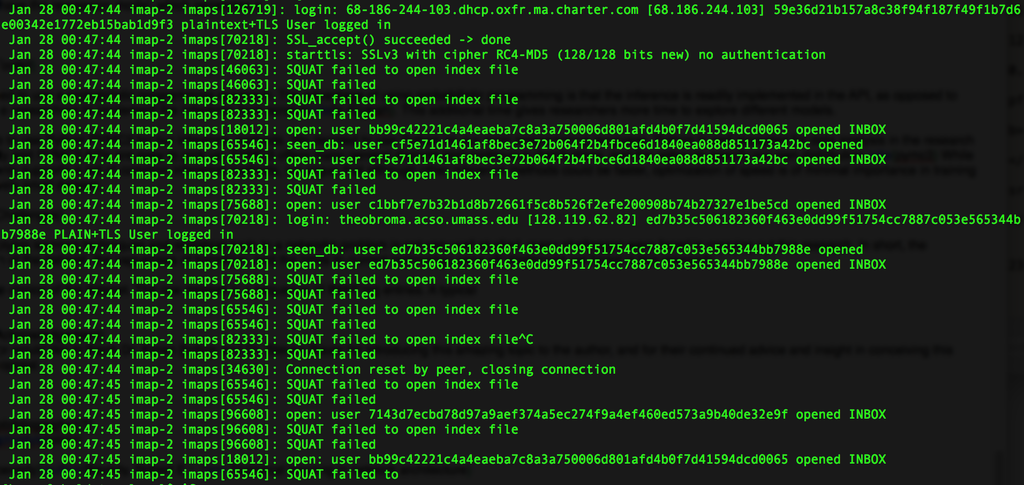
\includegraphics[height = 7cm, width =15cm]{imapSample.png}
 \captionof{figure}{Sample IMAP entry for 2014.01.28}
 \end{Figure}
 
This is what a section of a sample IMAP processed logs file looks like. The most useful information here is that on line 1, a user with an IP address of 68.186.244.103 attached to the network. In the middle section, another user attached to the UMass network. At 00:47:44, the server unilaterally detached the idle user identified by 34630. The log also includes information on when the user checks the inbox and deletes messages. Note that the user identity, which is originally an email address, is masked using SHA2-hashing \cite{yang} to protect user privacy. 

We may further extract the device the user signed in with, and acquire additional information from the IP address. We used the free website \textit{ip-api.com} to determine the user's city location and internet service provider (ISP) information. We threw out entries that have unidentifiable IP addresses, and entries with abroad IP addresses. Those entries account for roughly 3\% of the entire dataset. 

We note that a user can simultaneously be signed into the same email account from multiple devices or networks. The server does not dismiss a user's first attachment once s/he signs in from a second device.


\subsection{Markov Chain For Transition Prediction}

One of the important results in Yang's paper is a 3-state Markov chain model that predicts the likelihood of a user transitioning, given the number of networks s/he is currently on.

To understand how users make network transitions, first we need to define a transition.

\begin{definition}
A \textbf{session} is a continuous period of time for which a user is on the same network, which is defined by the same IP address. A \textbf{transition} happens when the user detaches from one network and attaches to another one.
\end{definition}

With this definition, we can decide whether a transition happens from the logs. Brian Copeland, a UROP student of the ANA group, parsed the original UMass log entries into SQL entries that contain each individual session. We overlay the durations to decide occurrences of transition. The details of transition criteria can be found in Yang \cite{yang} paper.

A Markov model is a way of modeling the randomly changing systems where the future states only depend on the current state. There are four types of Markov models depending on two criteria. Observable evaluates whether the state of the system is directly observable by the outside. Controlled means for each new step, the system has options on which action to take, and this action affects the transition probabilities. Autonomous means that the system does not have the option to choose an action. 

\begin{center}
    \begin{tabular}{| l | l | l |}
    \hline
     Dimension& System State Fully Observable & System State Partially Observable \\ 
    \hline
    System is Autonomous & Markov Chain &Hidden Markov Model(HMM)\\ 
    System is Controlled& Markov Decision Process(MDP) &Partially Observable MDP\\ 
    \hline
    \end{tabular}
\captionof{table}{Different kinds of Markov Models\cite{markov}}
\end{center}

In Yang, the researchers implemented a Markov Chain, that is, a system with fully observable states and no action options. The three states of the Markov chain are 

\begin{itemize}
\item
On 0 networks
\item
On 1 network
\item
On $\geq 2$ networks
\end{itemize}

A 3 by 3-state transition probability matrix can be calculated directly from the dataset. One subtle choice we have to make is how often we call each time step. One extreme is to take near-continuous measurements. For instance, we can consider every second as a new time step. However, this creates an inescapable state. On average, a typical user logs 20 sessions a day. There are 86400 seconds in one day. This is at most 20/86400 = 0.23\textperthousand. Hence we are likely to be stuck in the on 0 networks state. Using such a model, we might create a skewed dataset that does not faithfully captures the original.

We took measurements at the end of each 20-minute period as Yang claimed 20-minute periods was optimal for this dataset \cite{yang}. We look at the networks the user is on at the end of the 20-minute window, versus at the beginning, to see whether s/he has transitioned. In table 2, we have the transition probability matrix calculated on a 10000 user days training sample. Given this transition probability matrix, we can generate estimations of what the user may behave in the future. We then compare this model generated data with the testing sample.

\begin{center}
    \begin{tabular}{| l | l | l | l |}
    \hline
     Transition Prob.& On 0 Networks & On 1 Network & On $>=1$ Networks\\ 
    \hline
    On 0 Networks CRF& 0.930 &0.066 & 0.004\\ 
    On 1 Network& 0.696 &0.266 & 0.038\\ 
    On $>=1$ Networks & 0.291 & 0.356 & 0.353\\
    \hline
    \end{tabular}
\captionof{table}{Empirical estimates of transition probabilities. Data acquired on training sample (10000 user days).}
\end{center}


\subsection{Evaluate Markov Chain Prediction}

For baseline, we evaluate the distribution of the number of transitions for all users on a daily basis as noted in Yang. We identify a transition as a change of state (on 0, on 1, or on 2 or more) from the end of the previous 20-minute period to the end of the current 20-minute period. We compute one distribution from the testing dataset, and another for the randomly generated dataset based on Markov chain runs. We make the simple assumption that all users behave similarly and the transition distributions are approximately normal. 

\begin{Figure}
 \centering
 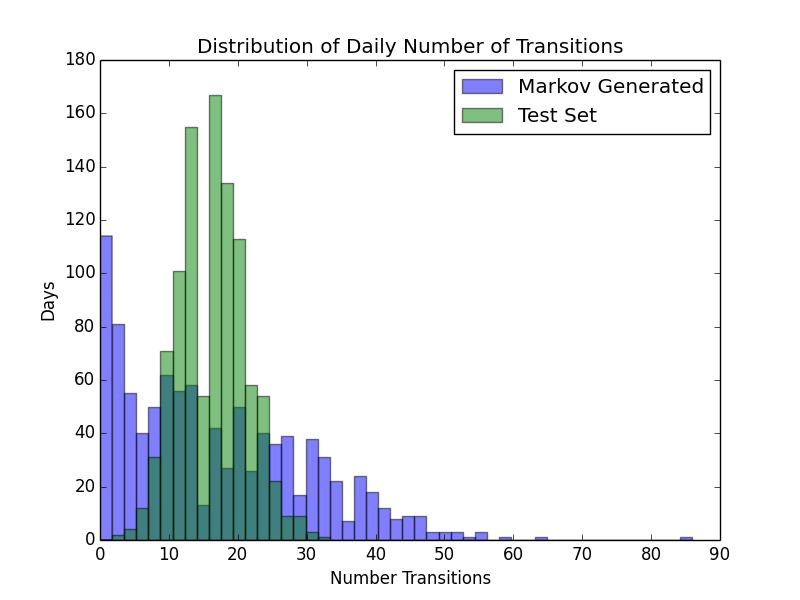
\includegraphics[height = 11cm, width =15cm]{figure_1.png}
 \captionof{figure}{The distribution of number of transitions from Markov chain and testing set. Sample size 1000 user days each.}
\end{Figure}

In figure 3, we illustrate the distribution of daily transitions for 1000 sample days generated by the Markov chain and 1000 days from the testing data. The testing data shows a more Gaussian distribution, whereas the Markov chain generated data shows a skewed tail. Despite the two datasets having similar transition probability matrices, the Markov chain failed to capture the normal distribution. This is similar to the concern exhibited before. The probability matrix created a 0-state that generated data might get trapped into. We confirm the concern that a simple three state Markov transition matrix alone does not perfectly capture the transition behavior exhibited by the dataset.

\subsection{Aspects of Modeling where Markov Chain Falls Short}
We do not believe that such modeling optimally captures user behavior for the following reasons.

\begin{itemize}
\item
Loss of information by the probability matrix.

By categorizing the user into one of the three states, we assume the transition only depends on the number of networks a user is on. The user's likelihood to make a transition can depend on other factors, such as how long s/he spends time on the current network.

\item
Loss of individuality of users

The entire dataset contains users of various habitual patterns. There could be a number of groups of users who have contrasting transition probability matrix. By combining all users together, we only gain insight on how an "average user" behaves like, though this "average user" may be a mix of several exemplary users.

\item
Failure to capture the normal distribution

The Markov chain generated dataset presented a more exponential distribution of transitions, as opposed to normal distribution in the test dataset.
\end{itemize}

We continue to the next section to evaluate what can be done along those dimensions.


%device???

\subsection{Questions that Emerge from Yang Experiment Reproduction}

Due to the simplicity of the Markov chain, we can ask several major questions: 

\begin{itemize}
\item
Can the entire user population be broken down into groups? How many different groups of users are there? 
\item
How frequently do users transition? What does a typical transition look like? What factors can signal, or affect a transition?
\item
Do users exhibit any periodical behavioral patterns?
\end{itemize}

We first answer the grouping question by utilizing clustering algorithms.


% This chapter can be redone by starting from a markov model approach, then explain the ups and downs that lead to 

%The approaches used here are

%\begin{itemize}
%\item
%Markov Model
%\item
%Regression
%\item
%Probabilistic Programming
%\item
%Clustering
%\end{itemize}

\newpage

\section{Modeling}

\subsection{Clustering Finds Three Groups}

A closer inspection at the dataset conceives the idea that we may split the user into user groups. The population in the dataset is residents of UMass. This could include professors, students, and other populations whose behavioral pattern are vastly different. It would be beneficial for the algorithm to take separate inferences for each one of the groups. 

We used K-means analysis for carrying out the clustering analysis. K-means analysis is a commonly used clustering algorithm that is scalable and fast. A typical implementation of the k-means algorithm needs the user to provide the number of clusters, or $k$. The algorithm then picks the $k$ initial starting centroids for the population, and gradually update the position of centers as the algorithm iterates itself. In Tibshirani\cite{tibshirani}, the optimal number of clusters $k$ can be found using the gap statistic, which finds a statistic to measure the comparison of the compactness of the clusters with a distribution of no obvious clustering. We implemented such an algorithm with features including ID, IP, start time, end time, average session duration, Android, Apple, device, whether the ISP is wireless, whether the ISP is wifi, and average number of sessions per day. Three clusters were identified by the algorithm. This clustering separates the users mainly by average session durations. 

\begin{Figure}
 \centering
 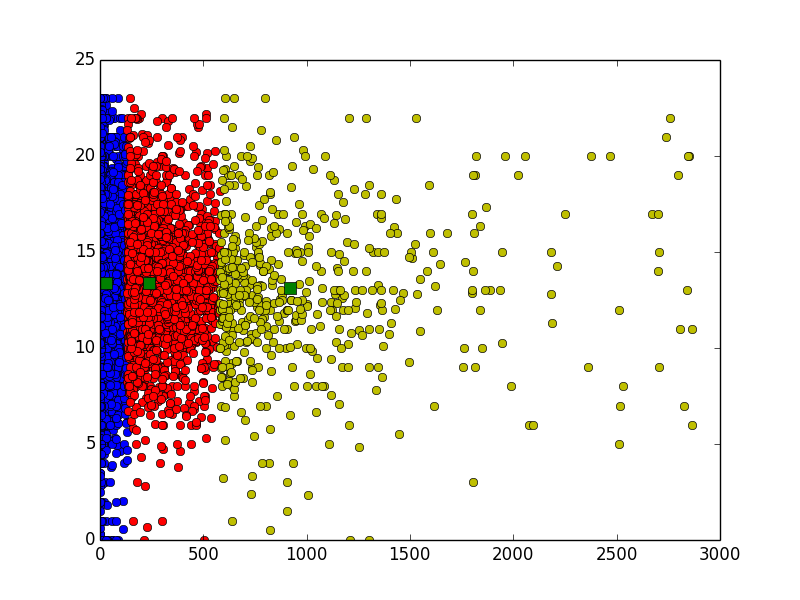
\includegraphics[height = 8cm, width =12cm]{3ClusterKMeans.png}
 \captionof{figure}{The clustering algorithm output. X-axis is average duration in seconds. Y-axis is session start hour. Average duration length significantly affected the clustering. The green dots represent the centers of each cluster.}
\end{Figure}

\begin{Figure}
 \centering
 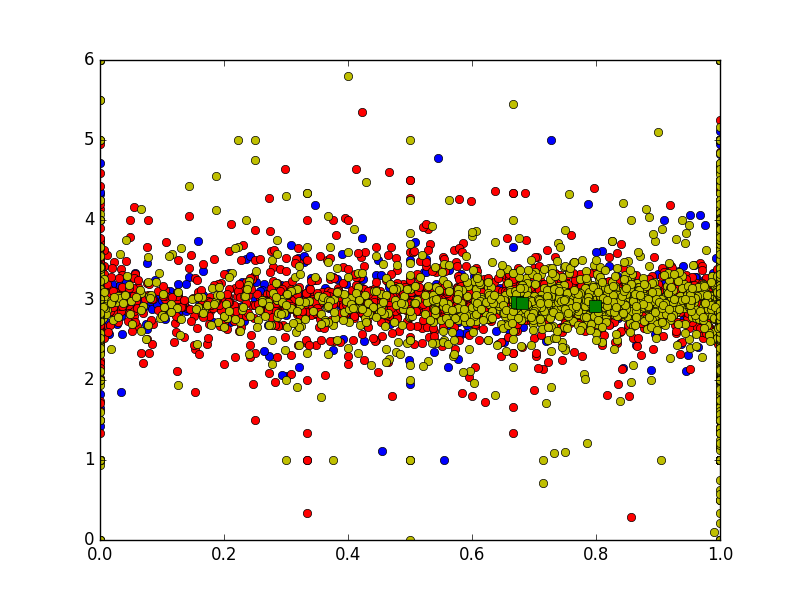
\includegraphics[height = 8cm, width =12cm]{cluterWifiWeekday.png}
 \captionof{figure}{X-axis is portion of user entry being from a wifi ISP. Y-axis is day of the week. Those were two of the features that did not significantly affected the clustering.}
\end{Figure}

\begin{Figure}
 \centering
 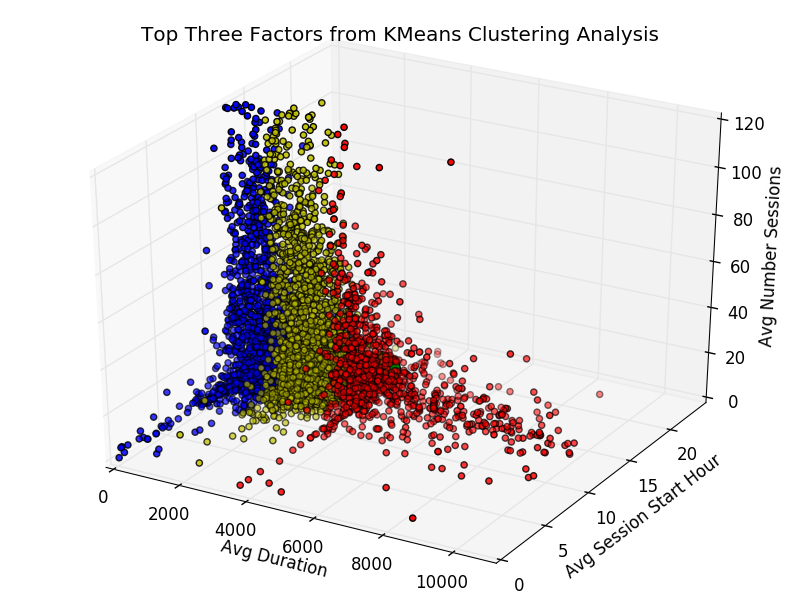
\includegraphics[height = 9cm, width =12cm]{Threefactorclustering.png}
 \captionof{figure}{The K-means clustering algorithm output. The top three factors for separating the dataset are average duration per session, average number of sessions in one day, and the average starting hour for sessions.}
\end{Figure}

The K-means clustering algorithm helps quantify the influence each feature has on dissecting the dataset. Here the k-means algorithm proposes that average session duration is the number one factor for distinguishing user types. Another plausible but less promising factor is the average number of sessions on an average day.

The researcher makes the following arguments and observations regarding this output.

\begin{itemize}
\item
The long duration cluster transitions less frequently.
\item
Users with on average long durations may be less likely to transition.
\item
The number of sessions per day can directly affect the calculation of how frequently the user transitions.
\item
Users who have on average short sessions and high number of transitions tend to switch between networks more frequently. Hence when designing a new network to maximize efficiency, those users deserve extra attention for congestion.
\end{itemize} 

We move on to test the arguments above.

\subsection{Clustering Shines Light on Canonical User}

To test out the hypotheses above, we break the users into clusters, and then calculate the Markov transition probability matrix to see whether there is a significant difference.
%%THIS SUBSECTION NEEDS CLARIFICATION AND EXPANSION

\begin{center}
    \begin{tabular}{| l | l | l | l |}
    \hline
     Transition Prob.& On 0 Networks & On 1 Network & On $>=1$ Networks\\ 
    \hline
    On 0 Networks CRF& 0.930 &0.066 & 0.004\\ 
    On 1 Network& 0.696 &0.266 & 0.038\\ 
    On $>=1$ Networks & 0.291 & 0.356 & 0.353\\
    \hline
    \end{tabular}
\captionof{table}{Empirical estimates of transition probabilities for all users.}
\end{center}

\begin{center}
    \begin{tabular}{| l | l | l | l |}
    \hline
     Transition Prob.& On 0 Networks & On 1 Network & On $>=1$ Networks\\ 
    \hline
    On 0 Networks CRF& 0.896 &0.096 & 0.008\\ 
    On 1 Network& 0.694 &0.266 & 0.040\\ 
    On $>=1$ Networks & 0.285 & 0.293 & 0.422\\
    \hline
    \end{tabular}
\captionof{table}{Empirical estimates of transition probabilities for the long duration cluster.}
\end{center}



\begin{hyp}
The average user in the long duration cluster (average duration $\geq67\%$ percentile) exhibits on average less number of transitions than the average user.
\end{hyp}

$H_0$ is that the average user in the long duration cluster exhibits on average the same number of transitions as the average user.

First we see that on average, the long duration users have a daily 18.49 sessions, whereas the average user of the population of 6084 has a daily 20.64 sessions. The result is significant $(p=0.00179)$ by the t-test. So we reject the null hypothesis.

\begin{Figure}
\centering
 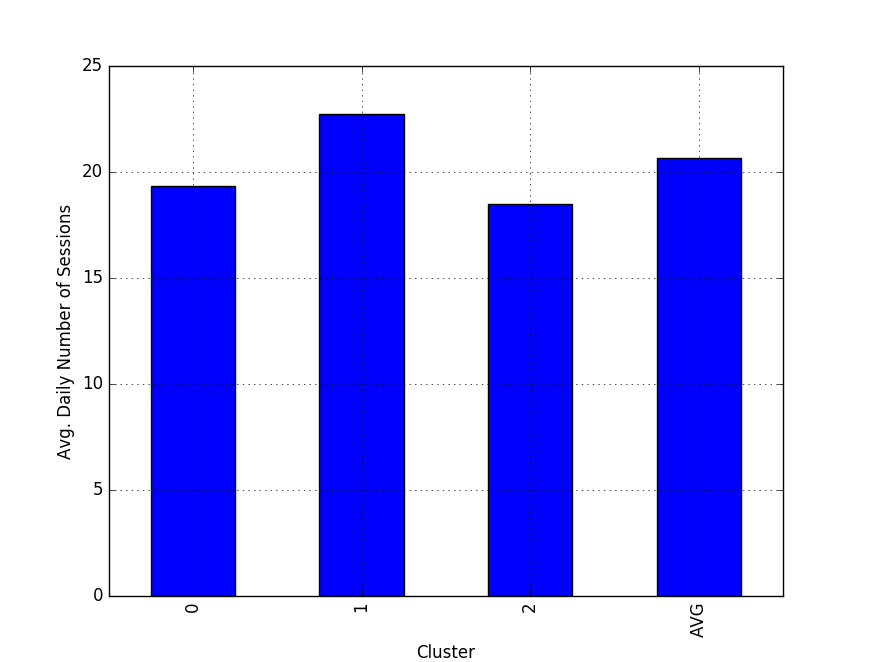
\includegraphics[height = 6cm, width =9cm]{clusteredAVGNUMSESSION.png}
 \captionof{figure}{The average number of sessions per cluster.}
\end{Figure}

\begin{hyp}
Users with on average the 1/3 most sessions per day transition more frequently than the average user.
\end{hyp}

By using a similar t-test, we observe that users with more sessions group on average transition

After calculating transitions as defined in section 4.1, we obtain the following results.

[Here add some material on acknowledging the hypothesis, especially revise the code to check whether number of transitions is different.]

\subsection{Regression Helps Weighing Factors}

The second downside of the Yang model is that it assume the user's current state as the only factor that decides the transition. We'd like to quantify the effect each feature has on the transitioning.

To answer the question how frequently do users transition, there are several parameters we can model. We chose to model for each user, how many sessions happened in a given day, and what is the duration of each session. If we can accurately model the number of sessions in a day, how long each sessions is, and when exactly these sessions happen, then we can overlay the sessions to evaluate the transitions.

We first tried out with regression analysis. Regression analysis evaluates the relationship between a dependent variable and multiple independent variables. It does so by creating a curve that fits all the data points with minimal total error norm. We started out by exploring linear regression models for simplicity. More specifically, let each $x_i$ be a $p$-dimensional feature vector for prediction, for each $y_i$ the prediction values, a typical regression estimates $\beta$ by minimizing

\begin{equation}
\sum_{i}{(y_i - x_i^T\beta)^2},
\end{equation}

where $\beta$ is the weight vector for the variables. 

Regression analysis can be used to discover correlations between the variables. One of the challenges of our dataset is that the predictors are not entirely independent. Hence we tried Ridge regression and Logistic regression.


\subsubsection{Ridge Regression}

\paragraph{Background}
Ridge regression is a technique that evaluates multiple regression data that suffer from multicollinearity\cite{ridge}, or multiple predictor variables being highly correlated. Ridge regression resolves that issue by \textit{regularization}, or adding a penalty on the weight sizes. Specifically, let each $x_i$ be a $p$-dimensional feature vector for prediction, for each $y_i$ the prediction values, Ridge regression estimates $\beta$ by minimizing

\begin{equation}
\sum_{i}{(y_i - x_i^T\beta)^2 + \lambda\sum_{j=1}^p{\beta_j^2}},
\end{equation}

where $\beta$ is the weight vector for the variables, and $\beta_j$ is the weight vector for the $j$th variable. The first sum calculates the error term, and the second sum creates an additional penalty on the absolute size of the individual weights. This partially resolves the multicollinearity of the variables. If two variables are negatively correlated, the additional regularization term pushes the weights to small absolute values\cite{bishop}. Note that there is an additional regularization constant $\lambda$, which controls how much having weight values of small absolute values matters. The choice of $\lambda$ is due to the researcher and trial and error.

\paragraph{Results}
\paragraph{Predicting Session Duration is Difficult}

First we looked at the general user population. We used scikit-learn as our library, for its ease of use and availability of tutorials. We passed in 5 million entries of session data, where each entry $x_i$ consists of user ID, IP address by bits (32 bits), timeStartBucket \{0 - 23\}, day of week, device, whether the device is Apple, and whether the device is Android. Each $y_i$ is the duration of the session. We used a set of $\lambda$ values $[0, 0.001, 0.01, 0.1, 0.2, 0.5]$. Note that setting $\lambda$ equal to 0 is equivalent to not having regularization.

\begin{Figure}
 \centering
 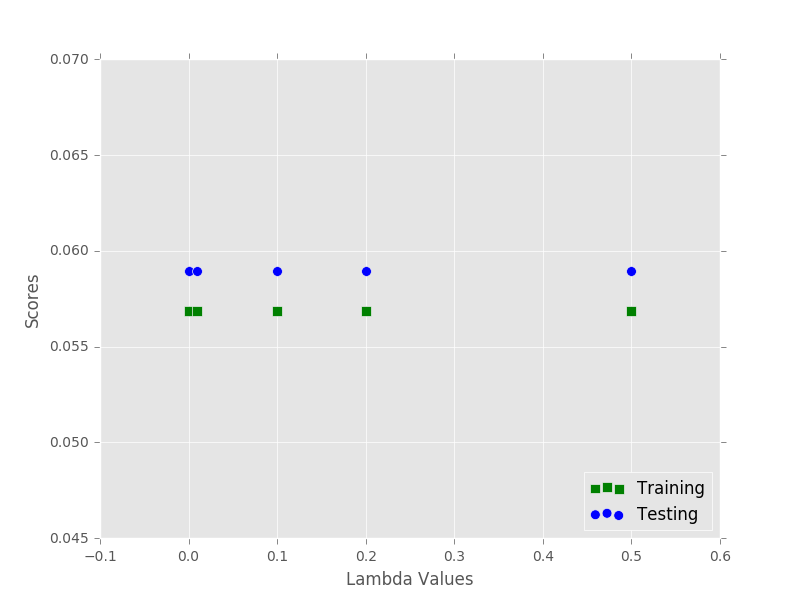
\includegraphics[height = 7cm, width =10cm]{ridgeScores.png}
 \captionof{figure}{Ridge Regression Scores. Lambda values do not significantly affect performance.}
\end{Figure}

Using this dataset to train, we tried to make predictions on the session duration of the remaining 2.5 million available entries. Unfortunately, we reached terrible scores ($<10\%$) on both the training and testing dataset for Ridge regression. 

Puzzled, we revisited the distribution of the durations. 

\begin{Figure}
 \centering
 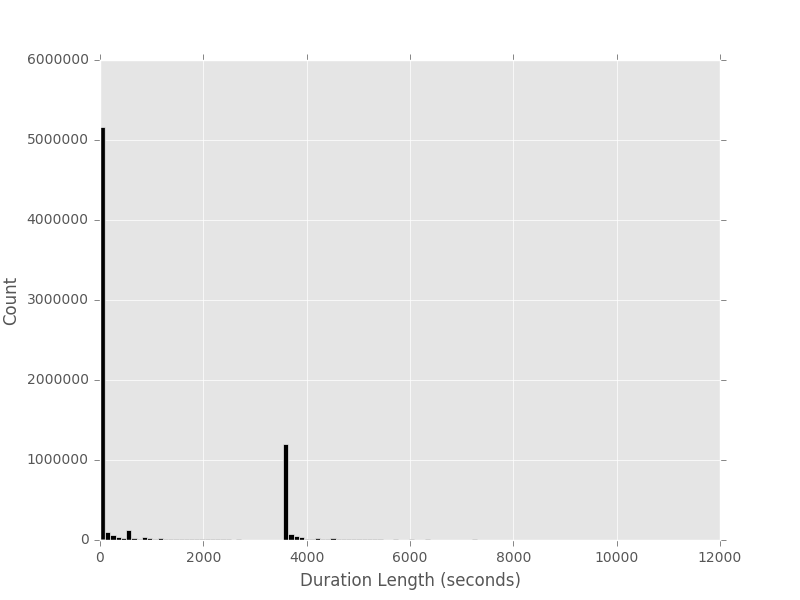
\includegraphics[height = 7cm, width =10cm]{durationDistribution.png}
 \captionof{figure}{The distribution of session durations, in seconds. Note the second peak at the hour mark.}
\end{Figure}

We observe there is a secondary peak at the hour mark. A deeper inspection at the original processed dataset reveals that a supermajority of those session connections were closed by the server after an hour of idle time. This does not conflict with our definition of session, as the user was \textit{on}, despite not utilizing the network, for the entire time.

The results show that the features we used cannot distinguish whether a duration is going to be less than a minute or an hour long. Because the prediction is linear, the results easily become bizarrely off. We then examined other statistical approaches that can better capture this discontinuous distribution of the dependent variable.

\paragraph{Predicting Number of Sessions}
%% HERE

We separated the user into three clusters as found by the k-means algorithm above. For each cluster, we implemented a Ridge regression model to predict the number of sessions for each day. The features used were whether the device is apple, whether the device is android, what day of the week it is, the user's likelihood to be on a wireless network that day, average duration for this user's sessions, average session start time for this user.

The main observations are:

\begin{itemize}
\item
Using just the features provided with a linear regression model cannot predict the number of sessions in a given day
\item
Being on a wireless network decreases the number of sessions per day. Being on a wifi network increases the number of sessions. This is potentially due to the automatic email checking is only on when on a wifi network to save wireless data usage.
\item
Grouping by cluster does not help that much. 
\end{itemize}

Note that in predicting the daily number of sessions, we are no longer accessible to the unique IP address as found in each entry before. This decrease in number of independent variables further decreased the performance of our prediction. 

[TODO: Address how the algorithm calculates the test/training scores]

\begin{Figure}
 \centering
 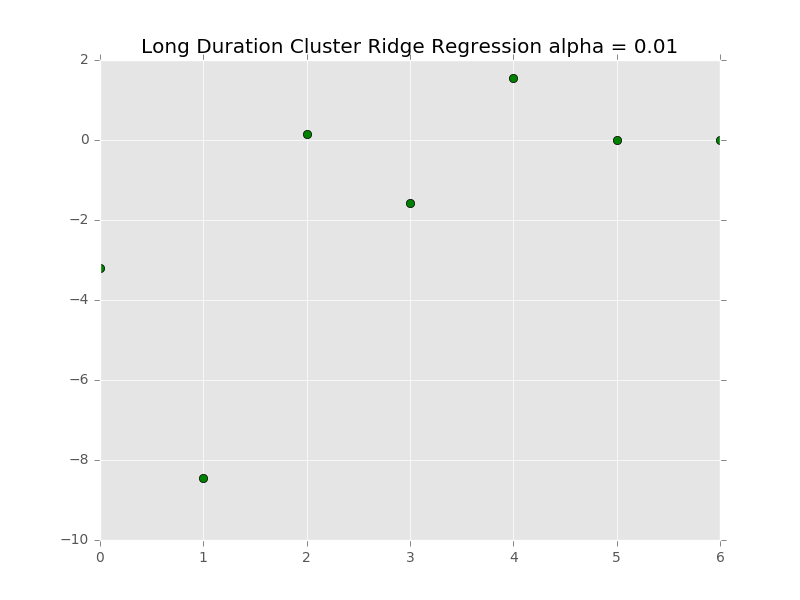
\includegraphics[height = 7cm, width =10cm]{c3avgses.png}
 \captionof{figure}{The long cluster average session length prediction. Each $x_i, i \in \{0,1,2,3,4,5,6\}$ is a parameter and the y-axis is showing the variable's corresponding weight.}
\end{Figure}

Scores on the training dataset and testing dataset were around 7\% accurate. This result serves as a baseline and opens up discussion for alternative modeling techniques. Training the model took 0.002 seconds on average due to the low dimensions.

\subsubsection{Logistic Regression}

\paragraph{Background}

Since Ridge regression performs poorly by directly predicting the exact number of average sessions and duration length, we asked whether a categorical answer (such as long or short) can be acquired through regression. Logistic regression is a regression model where the dependent variable is categorical, as opposed to continuous. Logistic regression makes its predictions by comparing the likelihood of each individual category, and picks the category with the highest likelihood.

Formally, the logistic regression tries to predict the conditional probability $Pr(Y=1 | X= x)$, where $Y$ is the binary indicator variable for the category (0 or 1). In order to reach a 0 or 1 output, we need to carefully examine the math to produce the correct results.

The formal model \cite{cmulogisitc} is that

\begin{equation}
log\frac{p(x)}{1-p(x)} = \beta_0 + x\cdot \beta
\end{equation}

where $\beta_0$ is the $y$-intercept and $\beta$ the weights for the features. Solving for $p$ we get

\begin{equation}
p(x) = \frac{e^{\beta_0 + x \cdot \beta}}{1 + e^{\beta_0 + x \cdot \beta}} = \frac{1}{1 + e^{-(\beta_0 + x \cdot \beta)}}
\end{equation}

To minimize error, we should predict $Y=1$ when $p \geq 0.5$ and $Y=0$ when $p < 0.5$. This means predict 1 when $\beta_0 + x \cdot \beta \geq 0$, 0 otherwise.

We used a variation of the logistic regression model, namely we expanded it to predict from multiple categories. That is,

\begin{equation}
Pr(Y=c | X = x) = \frac{e^{\beta_0^{(c)}}+x\cdot \beta^{(c)}}{\sum_c{e^{\beta_0^{(c)} + x\cdot \beta^{(c)}} }}
\end{equation}

Instead of having one set of parameters $\beta_0$ and $\beta$, each class $c$ has its own offset $\beta_0^{(c)}$ and weight vector $\beta^{(c)}$. The remaining calculations are analogous as the binary case. The category $c$ with the highest probability gets picked.

\paragraph{Results}

We used scikit-learn as our library for its readily implemented multi-class logistic regression module. We passed in 5 million entries of session data, where each entry $x_i$ consists of user ID, IP address by bits (32 bits), timeStartBucket \{0 - 23\}, day of week, device, whether the device is Apple, and whether the device is Android. We further broke duration into short ( $<$ 5s), mid (5s - 60 mins), and long ( $>$ 60 mins). The cutoff at 60 minutes is because we noticed a peak at slightly more than 60 minutes for duration distributions.

\begin{Figure}
 \centering
 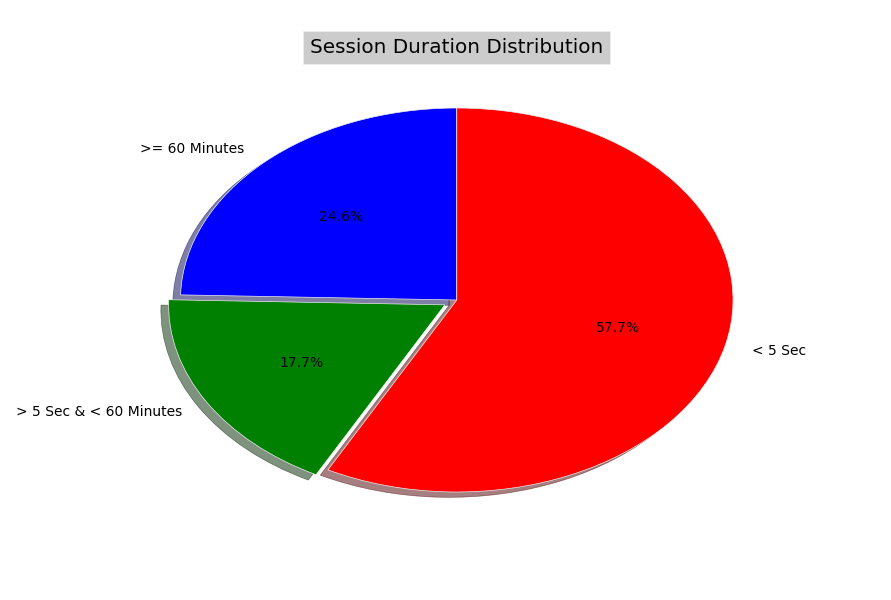
\includegraphics[height = 9cm, width =10cm]{durationDistPie.png}
 \captionof{figure}{The distribution of session durations, by tags.}
\end{Figure}


The Logistic regression predicts correctly the duration tag($y_i$=long, mid, or short) at $67\%$ accuracy, which is better than chance (1/3). Those values are far from accurate predictions. The features that carry the most weights are Apple or Android, and specific leading bits of the IP address. Having the device being Android produces more likely a long session. This naturally leads to questions like whether the Android's transfer protocol and app settings by default lets the user stay on a network for long periods of time without disconnection.


%Here a regression model was used to predict the number of sessions of each user per day. Since each user is different, we tried three approaches: 
%\begin{itemize}
%\item
%Treat all users as a uniform group. 
%\item
%Cluster users as user groups.
%\item
%Treat each user as a separate entity.
%\end{itemize}


[ADD SVM here]

\subsection{Neural Net Increases Performance}

\subsubsection{Background}

We see that the regression approaches have limited practicality as they suffered from the curse of dimensionality and specifically for our implementation, linearity. We also see that SVM suffered from slow training speed due to its large number of basis functions. Alternatively, we can fix the number of basis functions but allow them to be adaptive \cite{bishop}.

Neural network is one such approach that addresses the adaptiveness of basis functions. A neural net is very useful in problem domains where no known function for approximating the given features to their outputs. A neural net contains a collection of layers, where each layer has a collection of nodes. The input features are feed to the first layer and subsequently to next layers to run through mathematical calculation in an attempt to either condense or extract information. The end result is often a classification. The adaptiveness comes from its optimization of the mathematical calculations each round and in the activation functions used.

There are three general types of neural nets depending on the connection architecture of the nets\cite{neuralnetdesign}. 

\begin{itemize}
\item
Feed Forward Network
\item
Recurrent Network
\item
Reinforcement Network 
\end{itemize}

A feed forward network reads the input and feeds forward the information till the output produces a prediction. It is the simplest form of neural net. Such a net does not form a directed cycle in the network architecture. A recurrent network, on the other hand, can remember past inputs and forms a directed cycle in the network architecture. A recurrent net is useful in problem domains of natural language processing, in which the earlier part of the sentence is important in deciphering the meaning. A reinforcement network does not directly take input, but takes actions based on its environment and the reward function. Such an approach is often used in the robotics world.

\begin{Figure}
 \centering
 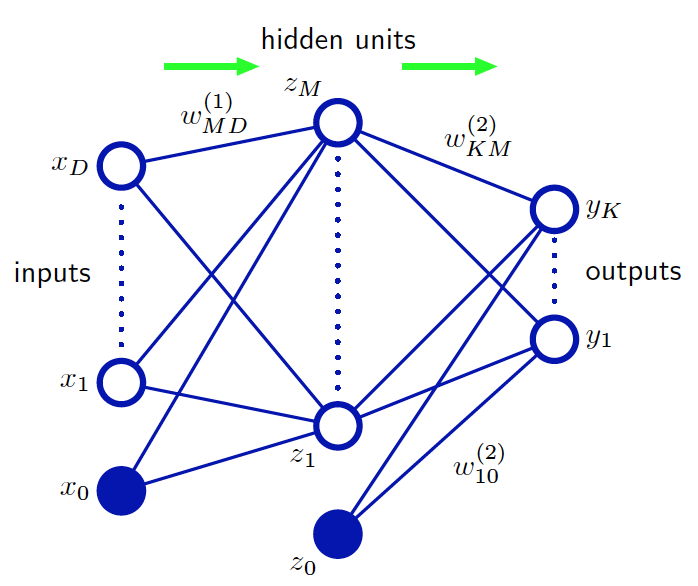
\includegraphics[height = 8cm, width =10cm]{neuralnet.png}
 \captionof{figure}{A one hidden-layer feed forward neural net. Image courtesy to Bishop\cite{bishop}.}
\end{Figure}

\paragraph{Mathematical Background}
The exact way neural networks carry out calculations may be less interesting, so readers can skip this section as needed. The one sentence summary is that neural networks specify an activation function, which can resolve nonlinearity.

Using the notation in the figure above, we have $D$ input data points, each data point $x_i$ contains its feature vector, and $M$ hidden nodes. The notations are due to Bishop\cite{bishop}.

\begin{equation}
z_j = h(\sum_{i=1}^D{w_{ji}^{(1)}x_i + w_{j0}^{(1)}}),
\end{equation}

where $h$ is a nonlinear activation function, $w_{ji}$ are the weights for the $i$th input and $j$th hidden node,  $w_{j0}$ is the intercept, or bias, for the $j$th hidden node, and superscripts (1) mean that the parameters are in the first hidden layer. The 

Similar operation happens from the hidden layer to the output layer. The activation function $h$ can be taken as the \textit{sigmoid} function, or

\begin{equation}
h(a) = \sigma(a)= \frac{1}{1+ e^{-a}},
\end{equation}

This sigmoid function turns a linear combination of input vectors into a nonlinear output. By taking this activation multiple times, the final output $y_k$ is no longer linearly related to the original input.

\subsubsection{Results and Discussion}

Since our main motivation is to increase performance on duration tag predictions, we implemented a feed-forward neural net with supervised training with one hidden layer.

With aid from Python's TensorFlow library, we implemented a one-hidden layer feed forward neural net with 7 features, 3 output nodes, and 10 hidden nodes. The features used were the same as in regression. The activation function is sigmoid and optimization was done using gradient descent. This net correctly predicts the duration tag with 83.4\% accuracy. The training and prediction took 633 seconds.

The results were not surprising to the researchers due to the following reasons.

\begin{itemize}
\item
The neural net has more parameters. The 10 hidden parameters created more flexibility for the model to better fit the outcome.
\item
The neural net has a nonlinear activation function. The duration tag is in no way linearly correlated with the features given. Hence resolving linearity largely increased performance.
\end{itemize}

[The Logically sound part ended here.]

%%%%END HERE

\subsection{Bayesian Modeling and Probabilistic Programming}
\subsubsection{Generative vs. Descriptive Modeling}

Despite the neural net having a high performance, we note that the neural net we used is mostly a classifier. That is, such an algorithm is an example of a descriptive algorithm. In general, modeling algorithms can be classified into two categories, generative vs. discriminative. A discriminative algorithm learns what criteria separate the classes given the dataset.  For instance, logistic regression is a discriminative algorithm. A generative model focuses on each class, and creates a model for what the underlying process for each class is \cite{ng}. Let $x$ be the feature inputs to the model, $y$ be the model output prediction, discriminative models learn $Pr(y | x)$, whereas generative models learn $Pr(x | y)$. That is, given the dataset, how likely is it that the data came from a distribution that is modeled by $y$. Therefore, generative model allows researchers to synthesize new dataset by understanding what the underlying distribution is. The Markov model is a generative approach, whereas regressions and neural nets are mostly descriptive models. We used the the discriminative approach when we needed to correctly classify or quantify parameters. To predict future actions, it is more practical to use a generative approach.

\subsubsection{Probabilistic Programming}

In this project we explored modeling using probabilistic programming, a kind of Bayesian modeling. Bayesian modeling creates a prior belief of how data \textit{should} look like before actually inspecting the dataset. Then, given the dataset, we produce a distribution for each parameter that we are interested in estimating, i.e. the posterior distribution \cite{ppblog}. Probabilistic programming is a way of inferring the ideal parameters for such modeling practice. It is a programming language as it abstracts away the mathematical calculations that goes on in inferencing the optimal parameters, just like a typical programming language abstracts away the storage of pointers in memory.

Roughly speaking, the steps involved in probabilistic programming are as follows:
\begin{itemize}
\item
Declare prior beliefs on what the data looks like.
\item
Feed in dataset.
\item
A sampling algorithm calculates a posterior distribution for each parameter in the model.
\end{itemize}

Probabilistic programming languages enable you to state your priors beliefs and your model with elegant, statistical syntax. Typically, the larger the dataset that's feed in, the less significant the prior beliefs become for learning the final parameters. In rare cases, the initial setup can produce local optimum that is impossible to climb out of. Hence it is recommended to examine several different prior beliefs. 

PP represents data and distributions with probabilistic parameters. Using a probabilistic programming approach gives estimation for parameters such as the mean of the normal distribution in distributions, as opposed to exact values. So PP makes statements such as "The mean of the normal distribution is normally distributed around 14 with a variance of 3.", instead of "the mean of the normal distribution is 14". This is beneficial as it can better capture the variance and other characteristics of shape.

We implemented a five factor model using probabilistic programming. Essentially, we are predicting two things, the number of sessions in a day, and the duration of an average session. We used Python PYMC3 as our API library. PYMC3 uses next-generation Markov Chain Monte Carlo sampling algorithms such as the No-U-Turn Sampler (NUTS) to sample its probability distribution \cite{pymc3}. Essentially, it constructs a Markov Chain that has the desired distribution at its equilibrium distribution, and uses Monte Carlo simulations to reach the approximation equilibrium. We can think of MCMC as similar to gradient descent in neural nets, which is a way of estimating the optimal parameters for the distribution. 

The pros for using PYMC3 include fast inference engine and simplicity to switch between distributions. PYMC3 offers NUTS and Hamiltonian Monte Carlo sampling, which works well on high dimensional and complex posterior distributions and allows complex models to be fit without specialized knowledge on fitting algorithms \cite{pymc3}. For instance, one can easily model the start time for each session as a normal distribution in PYMC3. Later, if one decides that a exponential distribution fits better, s/he can easily specify the desired shape for start time again.

\begin{Figure}
 \centering
 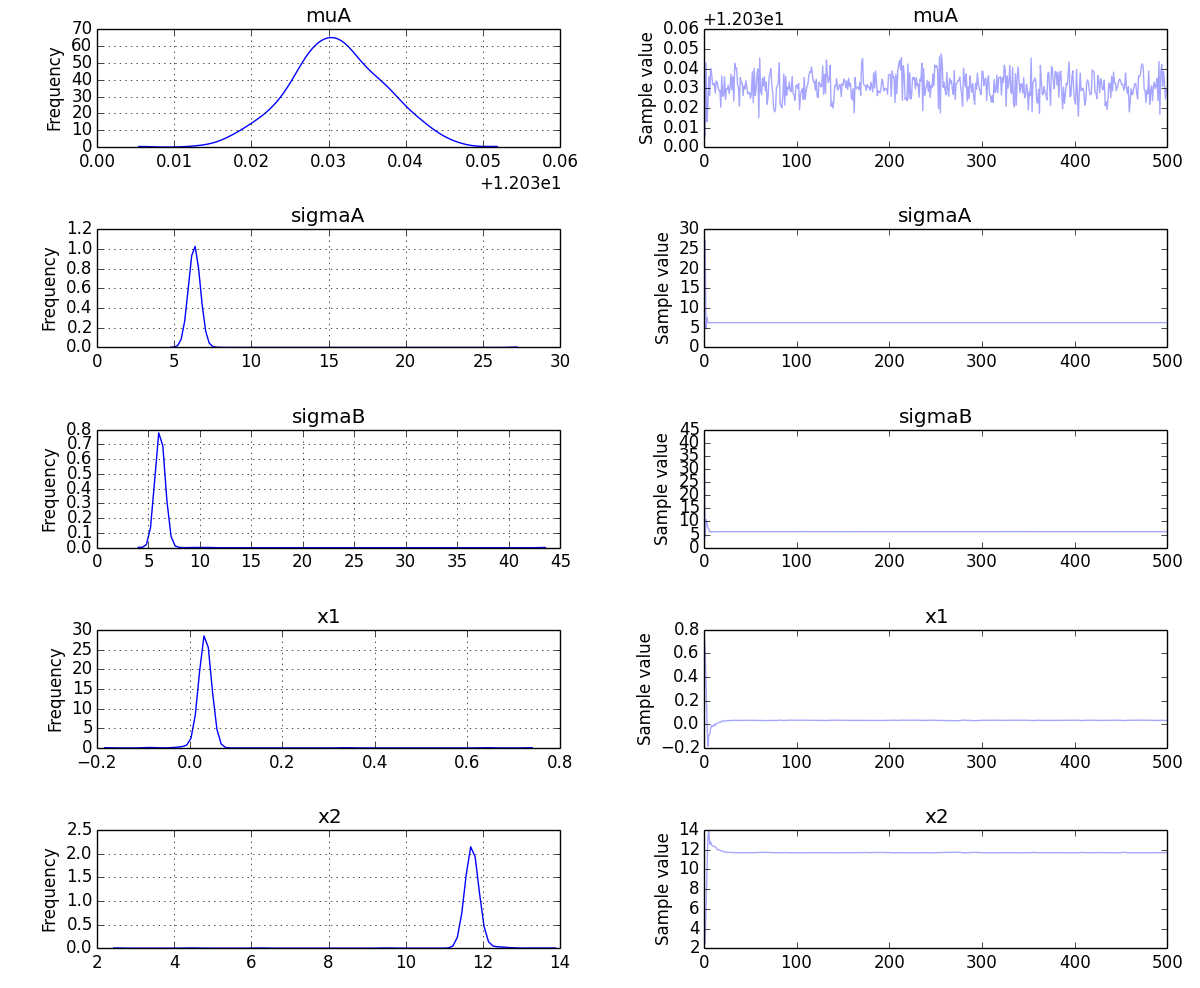
\includegraphics[height = 10cm, width =12cm]{ppsample.png}
 \captionof{figure}{An example PP output using PYMC3. A is the distribution of start times of a typical session, which is modeled as normal. We see that the mean is normally distributed around 12.033 with $\sigma$ of approximately 6. The right column shows each sampled $\mu$ and $\sigma$ values over the 500 sample Monte Carlo trials.}
\end{Figure}


With this approach, we implemented a duration prediction as a combination of two normal distributions, with a switch point. Switch point happened at 1800s, where the later normal has mean 3466 second, the earlier normal has mean 3.53 seconds. This approach is done on the general user population, hence it remains unclear what exactly are the factors that can cause the switch between long and short durations. 

Notably, we spent a lot of time in vein tweaking around the API to analyze more sophisticated, multiply dependent models. Please see challenges to see the lessons learnt related to PYMC3 and probabilistic programming.

\subsection{Failure to Capture Normal Distribution}


\newpage
\section{Evaluation}

\subsection{Approach Comparison}

This project gives the author a much more thorough understanding on what approaches are plausible for a networks dataset. We explored clustering algorithms, regressions, neural nets, and probabilistic programming.

We evaluate the pros and cons of the different approaches along three dimensions: prediction accuracy, speed of convergence, relevance to dataset.

\subsection{Speed}

In general, regressions are the fastest due to the simplicity of its models. A typical logistic regression finishes in less than 30 seconds, whereas training of a million entries in a one-layer feed forward neural net of 10 hidden nodes can take up to 10 minutes. Clustering varies its speed of convergence depending on the exact method. The K-means algorithm is relatively fast and takes less than a minute to converge.

\begin{center}
    \begin{tabular}{| l | l | l | l |}
    \hline
     Approach& Calculation Complexity & Optimization Complexity & What\\ 
    \hline%%%%%%
    K-means Clustering& $i$ rounds &$O(nkd) \cite{kmeanscomplexity}$ & 0.004\\ 
    Ridge Regression& 0.696 &$O(n|W|^2)$ & 0.038\\ 
    Logistic Regression& 0.291 & 0.356 & 0.353\\
    Neural Net & 0.291 & 0.356 & 0.353\\
    Probabilistic Programming& 0.291 & 0.356 & 0.353\\
    \hline
    \end{tabular}
\captionof{table}{Complexity of different approaches.}
\end{center}

In general, a sophisticated neural net requires relatively thick datasets. That is, for each entry, we need more features than the available 10. 

A sophisticated neural net still remains the most fruitful approach. However a neural net decreases the importance of human decision in creating the models. If the human has no idea what is happening in the dataset, then a neural net may better assist him to explore the undiscovered possibilities. However, such an approach does not tell causation apart from correlation. Two features may be both positively affecting a tag, but really one of the two causes the other and the positivity of the tag. So, if we use a graphical model approach, i.e. bayesian probabilistic approach, the researcher can better specify the details of the models. 

Regressions, whether Ridge or logistic, trades speed for prediction accuracy. A typical regression finishes in less than 30 seconds, whereas training of a million entries in a neural net can take up to [IDK, half an hour, try again to be precise.] 

In all the approaches we took, we treated the models no more complex than a linear model. Ceteris paribus, we see that neural nets perform the best because it introduces hidden layers and extra parameters. This suggests that in all trainings we did, we did not have enough features and parameters to correctly tune for the results. The fundamental difference in the different approaches we take involve how much we understand the dataset. The specific probabilistic programming we did requires knowledge on the structure of the dataset. We need to additionally understand the structural dependence of the parameters.

This is somewhat due to the width of our dataset. For each entry, we have at most 10 parameters. Those 10 parameters do not necessarily have enough decision power over the prediction values we wanted to predict. Therefore, a neural net may be a better approach, as it introduces enough hidden parameters. Alternatively, we could introduce hidden intermediate nodes in the graphical models and connect them with corresponding nodes. However, such an approach proves to be overly complex beyond PYMC3 abilities. 

[This should be a large section]

\newpage
\section{Toolkit}

Multiple tools were used in carrying out this research. A quick list gives Python Pandas, Theano, PYMC3, scikit-learn. 

We decided to use Python as our main programming language. Python is well accepted for data analysis in the research community and the researchers have mastery on Python.

We decided to use a probabilistic programming approach. The advantage of using probabilistic programming is that the inference is readily implemented in the API, as opposed to burden the researchers to implement the inference from scratch\cite[p.4]{ghah}. This additional time gives researchers more time to explore different models. 

There are many probabilistic programming tools available currently, many under active development. The researcher of this project wanted to pick a tool that has a relatively small learning curve, a stable release and a sophisticated support platform. Hence all separately written programming languages were not out of scope. We chose to use Python PYMC3 for our probabilistic programming API. PYMC3 APIs are easy to pick up. PYMC3 offers many general discrete and continuous distributions, and the option to specify our own distribution.\cite{pymc3} While PYMC3 only supports a set of common inference methods, we argue that although other inference methods could be faster, optimization of speed is of minimal importance in training our relatively small dataset.

There are several alternative Python APIs for probabilistic programming, and we list their pros and cons.

\begin{center}
    \begin{tabular}{| l | l | l | l |}
    \hline
     PP Language& Learning Curve & Alpha Version Software & Support Platform\\ 
    \hline
    PYMC3 & Low &No & Mainly Python, Stackoverflow\\ 
    Stan& Low &No & Mainly R, Stackoverflow\\ 
    Venture & High & Yes & Correspondence with developers\\
    Picture & High & Yes & Correspondence with developers\\
    \hline
    \end{tabular}
\captionof{table}{Comparison of various Python probabilistic programming APIs.}
\end{center}

Both PYMC3 and Stan (pyStan) are python APIs, Venture and Picture are new programming languages developed at MIT specifically for probabilistic programming. All softwares are under active development, but PYMC3 has released multiple stable versions since 2013. Stan has been along for equally long, but it's mainly a R interface that has provided a Python package \cite{pymcstan}. Therefore we picked PYMC3 as our probabilistic programming language.

Pandas is a widely accepted data processing API in python data analysis and our researchers have gained previous proficiency in it. TensorFlow and scikit-learn are typical bundles for writing neural nets and regressions in aiding the data analysis. 

[Write more about the toolkit]

\newpage
\section{Challenges}

Since applying learning techniques and statistical tools to a networks problem is not very thoroughly studied in the field, many challenges were faced in carrying out this research. In short, the dimension of the dataset, the vagueness of transition, and the limits to current technology were all challenges we faced in this research.

First is the choice of the dataset. The raw dataset is a sequence of IMAP log entries. A typical sample entry looks like this.

\begin{Figure}
 \centering
 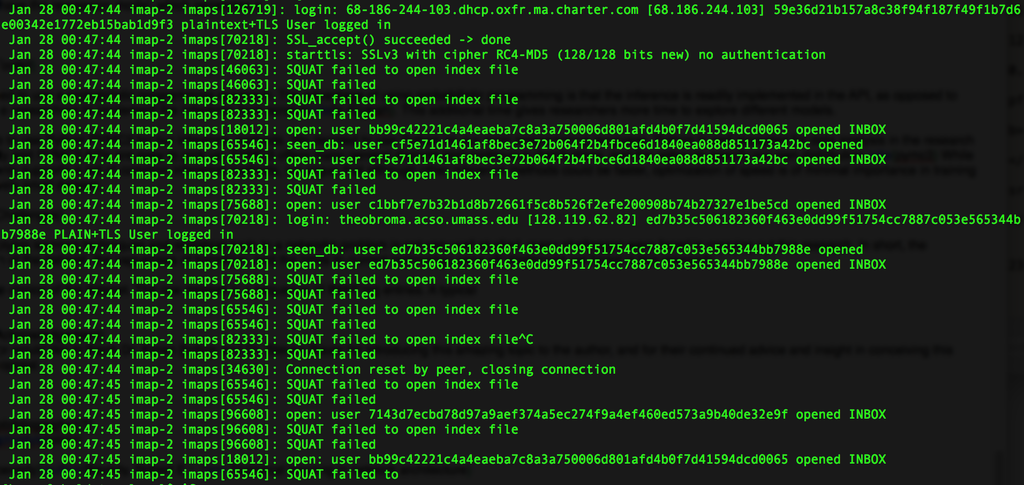
\includegraphics[height = 7cm, width =15cm]{imapSample.png}
 \captionof{figure}{Sample IMAP entry for 2014.01.28}
\end{Figure}

Here we see that the exact ending time for a session is hard to define, unless we see that the connection is reset by peer. In processing our datasets, we made the assumption that a user is on the network unless this network connection is explicitly closed or reset. This can introduce bias for users who were just on the network for a very short period of time but did not detach from the network. We make the argument that from the perspective of network design: since incoming data will still be directed to this idle but attached address, it is reasonable to consider the user as being on the network.

After processing, we have 12 million entries(lines) of sessions, as shown in figure.

\begin{Figure}
 \centering
 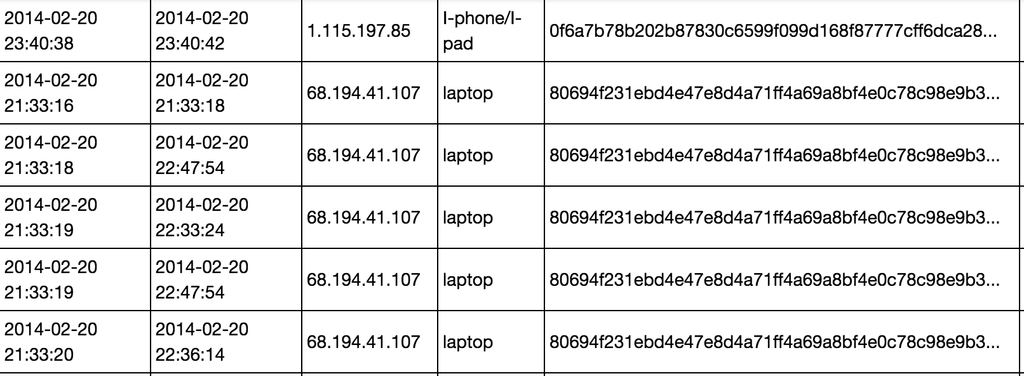
\includegraphics[height = 5cm, width =15cm]{dataSample.png}
 \captionof{figure}{Sample session data, each line is a session. The column headers are session start time, session end time, IP, device, user ID.}
\end{Figure}

This dataset is long but slim, so we went on a pursuit for other relevant features. We included indicator variables for Apple and Android. We included duration of each session, the day of the week, and the city, country, ISP of the IP address. We included an indicator variable for wifi vs. wireless network. Such features were meant to 1. help us achieve higher accuracies in prediction. 2. filter the dataset so that irrelevant data were dropped. While these variables are relevant, none of them is decisively important for our prediction purposes.

One of the major improvements that can happen is to pick a dataset and more carefully process the dataset. The current session definitions have issues regarding end times.

Another aspect of challenge is the technology. We chose to use PYMC3 for our API for probabilistic programming because we believed that probabilistic programming allows for flexibility in creating new models, but this API has its limits. 

One can break down ease of changing models in two cases, here we describe the process with a graphical model approach:

\begin{itemize}
\item
How easy is it to add new features (nodes)?
\item
How easy is it to change the distribution shape of current features (nodes)?
\end{itemize}

For the API we used, it is easy to change the distribution of a feature, but not so much to add a deeply connected node. In PYMC3, we can easily change the shape of the distribution to binomial, normal, Poisson, etc. due to its general inference engine. The NUTS and HMC sampler can easily readapt to the different shapes that we provide as the inference methods were already tuned. For each distribution class, a specific \textit{logp} method is written to facilitate the parameter estimation gradient calculations in NUTS and HMC sampling. Therefore it is very easy to switch models by means of changing distribution.

It is also easy to add new features, as long as the new feature is independent of other features. It is possible to do hierarchical bayesian modeling in PYMC3, but the API was not tuned for hierarchical inference. Working around the API requires hacks that slowed down the progress and incurred bugs that were not informative and difficult to fix. The algorithm returns errors for not being able to infer hierarchically dependent variables. In a neural network, we can specify an extra feature by adding in another column to the input vector / matrix. Even though the nodes can be dependent themselves, the user does not have to specify them. The actual causal dependence is not resolved, but the correlation will be discovered in the hidden layers, by ways of convolutional layers for dimensionality reduction. Such is not possible in PYMC3. We have to specify the graphical model for the variables first. If the parameters are dependent themselves, it is in the user's responsibility to figure out which parameter to infer first. If we change one node, we have to rewrite all other variables that is dependent on that node. This is a particular downside of PYMC3, by providing fast inference through Monte Carlo simulations, it sacrifices flexibility in structural dependency.

Another thing we learnt from applying probabilistic programming techniques is that the model needs to be clearly specified. The human expert needs to know exactly how A and B are linearly, exponentially, or otherwise dependent. In the ideal scenario, once the human feeds in data, the machine magically understand all the hierarchies and dependencies in data on its own, via a selection of possible dependence functions. This belongs to the field of structural learning, which is a more difficult problem. Tenenbaum \cite{tenenbaum} writes on the current state of hierarchical learning. In short, not only is it doing hill climbing in parameter space, but also in modeling space. The current technology seems to have limited grasp on hierarchical structural learning.




\newpage
\section{Contributions and Conclusion}

\subsection{Contributions}

The contributions of this thesis include 
\begin{itemize}
\item
Built and evaluated new models for network topological mobility.
\begin{itemize}
\item
Improved models and simulations of users mobile behaviors
\item
Utilized clustering algorithm to acquire canonical users
\item
Evaluated network mobility by user clusters
\end{itemize}
\item
Contribution to understanding of how network mobility affects new network design
\item
Use and demonstration of a suite of tools for broad exploration possibility.
\begin{itemize}
\item
Exploration of new modeling techniques and their application to networking challenges.
\item
Probabilistic programming
\item
Regression
\item
Neural Nets
\end{itemize}
\item
Compared and contrasted the different techniques used in the process.
\end{itemize}

\subsection{Conclusion}

Data analysis needs maturity and experience. By doing this project, I have acquired a much deeper understanding of the procedures and priorities of data analysis. The approaches taken to understand a dataset might be limited by the tools and dataset we have, but a good researcher can point the research in an insightful direction. Machine learning algorithms and statistical approaches can help provide additional understanding to the dataset if the researcher knows what factors are important but just don't know how exactly the factors are related. The first step in tackling a data analysis project is to understand what exactly to model for. Then, what exactly are the features that matter. Lastly, we pick the appropriate tools to explore.

\newpage

\begin{thebibliography}{20}
\bibliographystyle{plain}
  
\bibitem{beverly}\author{Beverly, Robert E.}. {\em Statistical learning in network architecture}

\bibitem{ghah}\author{Zoubin Ghahramani}. {\em Probabilistic machine learning and artificial intelligence} Nature, 28 May 2015.

\bibitem{jacobson} \author{Jacobson, Van}. {\em Networking Named Content} New York: Association for Computing Machinery, 2009.

\bibitem{ng}\author{Ng, Andrew}. {\em On Discriminative vs. Generative classifiers: A comparison of logistic regression and na�ve Bayes.}

\bibitem{yang}\author{Yang, Sookhyn}. {\em  Measurement and Modeling of User Transitioning Among Networks.}

\bibitem{kulkarni} \author{Kulkarni}. {\em Picture: A Probabilistic Programming Language for Scene Perception.}

\bibitem{find}\emph{NSF NeTS FIND Initiative} http://www.nets-find.net/

\bibitem{pymc3} PyMC3. https://github.com/pymc-devs/pymc3

\bibitem{tenenbaum} \author{Tenenbaum, Joshua}. {\em How to Grow a Mind: Statistics, Structure, and Abstraction.}

\bibitem{tibshirani} \author{Tibshirani, Robert. et al}. {\em Estimating the Number of Clusters in a Data Set via the Gap Statistic.}

\bibitem{ppblog} \author{Finkelstein, Noam}. {\em Probabilistic Programming for Anomaly Detection.}

\bibitem{pymcstan}\author{Carpenter, Bob}. {\em You'll never guess what's been happening with PyStan and PyMC.}

\bibitem{whyonlyus}\author{Berwick, Rob. Chomsky, Noam}. {\em Why Only Us: Language and Evolution.}

\bibitem{mobilityfirst}\author{Raychaudhuri, Dipankar}. {\em MobilityFirst Future Internet Architecture Project
Overview}

\bibitem{netsfia}{\em NSF FUTURE INTERNET ARCHITECTURE PROJECT}.

\bibitem{pporg} {\em http://probabilistic-programming.org/wiki/Home}

\bibitem{markov}\author{Kaelbling, Leslie} {\em Planning and acting in partially observable stochastic domains}

\bibitem{clustering} {\em http://scikit-learn.org/stable/modules/clustering.html}

\bibitem{ridge} {\em NCSS Statistics Software Ridge Regression}

\bibitem{bishop} \author{Bishop, Christopher} {\em Pattern Recognition and Machine Learning}

\bibitem{cmulogisitc} \author{Faraway, Julian} {\em Extending the Linear Model with R}

\bibitem{neuralnetdesign} \author{Hagan, Martin}. {\em Neural Network Design}

\bibitem{kmeanscomplexity} \author{Inaba, Mary}. {\em Applications of weighted Voronoi diagrams and randomization to variance-based k-clustering}

\end{thebibliography}

\end{document}
